\documentclass[12pt, letterpaper]{article}
\usepackage[utf8]{inputenc}
\usepackage{graphicx}
\usepackage{floatrow}

\usepackage[margin=2cm]{geometry} 



\renewcommand*\contentsname{Indholdsfortegnelse}

\begin{document}

\begin{titlepage}

\newcommand{\HRule}{\rule{\linewidth}{0.5mm}} % Defines a new command for the horizontal lines, change thickness here

\center % Center everything on the page
 
%----------------------------------------------------------------------------------------
%	HEADING SECTIONS
%----------------------------------------------------------------------------------------

\textsc{\LARGE Aarhus universitet}\\[1.5cm] % Name of your university/college
\textsc{\Large DSB}\\[0.5cm] % Major heading such as course name
\textsc{\large Semester 3}\\[0.5cm] % Minor heading such as course title

%----------------------------------------------------------------------------------------
%	TITLE SECTION
%----------------------------------------------------------------------------------------

\HRule \\[0.4cm]
{ \huge \bfseries Mini-projekt}\\[0.4cm] % Title of your document
\HRule \\[1.5cm]
 
%----------------------------------------------------------------------------------------
%	AUTHOR SECTION
%----------------------------------------------------------------------------------------

% If you don't want a supervisor, uncomment the two lines below and remove the section above
\Large \emph{Studerende:}\\[1cm]
Mette \textsc{Hammer Nielsen-Kudsk}\\[0,5cm] % Your name
Martin \textsc{Banasik}\\[0,5cm] % Your name
Finja \textsc{Jette Ralfs}\\[0,5cm] % Your name
%----------------------------------------------------------------------------------------
%	DATE SECTION
%----------------------------------------------------------------------------------------

{\large \today}\\[1,2cm] % Date, change the \today to a set date if you want to be precise

%----------------------------------------------------------------------------------------
%	LOGO SECTION
%----------------------------------------------------------------------------------------


\includegraphics[scale=0.5]{billeder/au}\\ % Include a department/university logo - this will require the graphicx package
 
 %\includegraphics[width=0.6\textwidth]{figurer/ASE}~\\[1cm]
%----------------------------------------------------------------------------------------

\vfill % Fill the rest of the page with whitespace


\end{titlepage}

\tableofcontents
\newpage

\section{Begreber}

Når vi går fra analoge signaler til digitale, så finder vi repræsentationer af det kontinuerer signal. Dette kalder vi samples og betegnes med N.
Når vi har flere samples på et signal, betegnes intervallet i mellem samples som $T_s$, samplingstid. Når vi har samplingstid kan vi indføre samlingsfrekvens, det inverse af samlingstid. $$f_s = 1/T_s$$
Så snart at vi har $T_s$, ved vi at vi har med et digitalt signal at gøre.

Ved opsætning af sampletidsaksen, definerer vi først vores sampletæller, $n$:
$$n = [0:N-1]$$ Hvor N er antal samples.
Efterfølgende bestemmer vi vores sampletidspunkter, $t$:
$$t = n*T_s$$
Vi kan nu indføre:
$$x(t_s) = X(n*T_s) = X(n)$$
Vi har altid en grundfrekvens og den kalder vi altid $f_0$.

\section{Aliasering}

Alias = et andet navn for noget/tvetydighed.
Vi har tre forskellige slags alias:
\begin{itemize}
\item Forkert samling - både for mange samples og for få
\item Gentagelser
\item Spejling (rundt om Nyquist-frekvensen)
\end{itemize}

Shannons sandheds sætning
$$f_s\geq 2*f_{øvre}$$
I praksis er dette aldrig lig med, men skal altid overholdes. 
Nyquist-frekvens:
$$f_{nyquist} = \frac{f_s}{2}$$
Altså defineret som halvdelen af samlingsfrekvensen, $$f_s$$

\section{Envelopes}

Envelopes = Amplitude billede over et tidsinterval. 
Under emnet evelopes har vi to punkter: 
\begin{itemize}
\item ADSR - Attack, Decay, Sustain, Release
\item LFO - Low-Frequency Oscillation
\end{itemize}


\section{ADSR}


Vi starter med ADSR: 
Her har vi en figur over den basale ADSR: 

\begin{center}
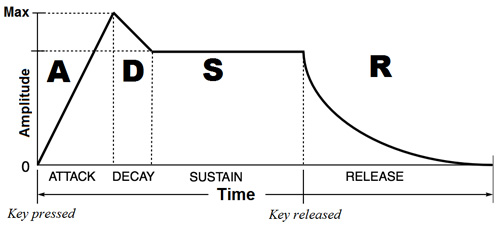
\includegraphics[width=\textwidth]{billeder/ADSR}
\end{center}

Som det ses af figuren har vi fire forskellige stadier: 
\begin{itemize}
\item Attack - Dette er i starten af signalet, hvor f.eks. en streng på en guitar bliver slået. Som vi kan se så stiger grafen kraftigt i Attack-stadiet. 
\item Decay - Her falder vores graf kraftigt, en smule, da vores streng på guitaren ikke kan holde den kraftige tone i så lang tid. Den skal falde ned til den stationære lyd, hvilket er det næste stadie.  
\item Sustain - Her holder vores graf et stationært niveau over noget tid. Dvs. at tonen, som vores guitar streng har givet, bliver holdt stabil over længere tid nu - Indtil tonen falder og dør ud (næste stadie). 
\item Release - Som vi kan se på vores graf dør vores signal ud her. Vores tone har altså holdt så længe den kan og dør nu ud efter det stabile-stadie. Så her falder og til sidst dør tonen ud. 
\end{itemize}


\section{LFO}

Hvis vi så går videre til LFO: 

\begin{center}
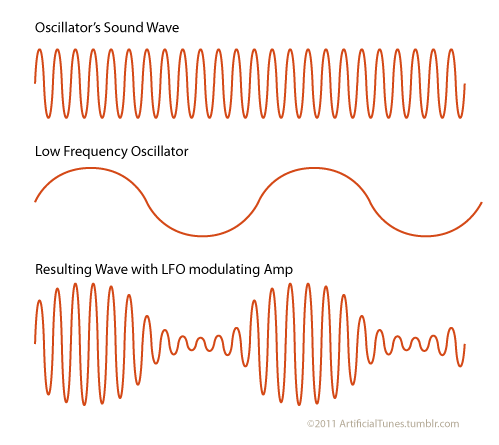
\includegraphics[width=\textwidth]{billeder/LFO}
\end{center}

Low-Frequency Oscillation er en anden måde at varierer amplituder på. 
Dette signal er for det meste under 20 Hz og bruges oftes til lydsignaler. Som navnet af denne metode siger, så bruger man altså kun dette når man har med lavere frekvenser at gøre. Frekvensen man benytter, når man skal have lavet sin sinusbølge, skal altid være lavere end tonen. 
Når man har fået lavet sin sinus kan vi beregne modeler sinus: 

$$S_{mod} (n) = (A_{vo} + 1)*s(n)$$
,hvor s(n) er vores sinus kurve. 

Herefter kan vi så beregne modulations graden, som betegnes, $f_L$.

Det skal så også siges at der er mange forskellige LFO-typer, det er ikke kun sinusser. Der er også firkants-, trekants-  og mange andre LFO-typer. 


\section{Fourier transformation}

I DSB har vi nogle forskellige analyse værktøjer. Et af disse er Fourier transformation (DFT). Når vi benytter DFT regner vi med komplekse tal. 
Definitionen af DFT er betegnet: 
$$X(m)= \sum\limits_{n=0}^{N-1} x(n)*e^{-j*\frac{2*\pi}{N}*m*n}$$

,hvor m = frekvens nummerering. 


Det er altså sådan vi går fra tidsdomæne x(n), til frekvensdomæne X(m) - via Fourier transformation, DFT. 

Hvis vi så gerne vil tilbage igen, altså fra frekvensdomæne X(m), til tidsdonmæne x(n). Så laver vi Invers Fourier Transformation, IDFT. 
Definitionen af IDFT er betegnet: 
$$x(n)= \frac{1}{N} \sum\limits_{m=0}^{N-1} X(m)*e^{j*\frac{2*\pi}{N}*m*n}$$

Længden er = 1. 
Herefter er vi altså tilbage i tidsdomænet x(n).

\section{Zero Padding}
Ved Zero Padding ligger vi x antal nuller ind i enden af vore signal. På den måde bliver længden af vores signal længere. Vi vinder altså ikke mere information omkring signalet, vi får blot flere "nuller-samples" hæftet på i enden. 
Dette gør at vi lettere kan fange frekvenskomponenternes opførsel (faktisk dobbelt så god frekvensopløsning) og at længderne på de forskellige signaler bliver ens. 
I dette miniprojekt synes vi ikke det gav mening, at lave Zero Padding på nogle af vores signaler og derfor er dette ikke blevet lavet. 

\section{Lækage}
Hvis man ikke rammer den rigtige frekvens ville alle ens samples fordele sig ud over hele x-aksen. Dette duer ikke, det bliver udoverskueligt og ulæseligt. Dette kaldes lækage. Lækage er noget vi kan få nedsætte ved hjælp af vinduer. (se næste afsnit). 

\section{Vinduer (Hanning Vinduet)}
Indenfor digital signal behandling har vi mange forskellige vinduer, der nedsætter lækage, ved hjælp af forskellige egenskaber. 
Hanning Vinduet er det vindue som vi benytter os mest af. 
Hanning Vinduet er energimæssigt mindre, hvilket ikke gør så meget, da vi let kan skrue op for strømmen. 
Vi mister frekvensopløsning - bliver faktisk næsten halveret, når vi benytter Hanning vinduet. Så vi betaler altså en pris, for at benytte os af Hanning vinduet, for at få vores signal til at se pænt og læseligt ud. 

\section{Udglatning (Smoothing)}
Udglatning fungerer lidt ligesom et lavpasfilter - det fjerner nemlig højfrekvenserne. 
Ved dette får vi altså pænere grafer, som er lettere læselige. Det er altså en udglatning af vores frekvensspektre, der er tale om. 

\section{Analyse}

Når vi laver sådan en analyse her så opstille vi to grafer: 
En for længden og en for fasen (Bodeplot). \\

\begin{itemize}
\item X-aksen = Frekvens i Hz (opdelt i decader)
\item Y-aksen på længde grafen = dB = $ 20*log(10)\mid X(m) \mid$ 
\item Y-aksen på fasevinkel grafen = $\angle (X(m))^{\circ}  $
\end{itemize}

Når vi har fået tegnet vores graf, så har vi det, der hedder Frekvensopløsningen, som er afstanden hver sample: 
$$\bigtriangleup f = \frac{fs}{N} $$

Det næste vi kan tilføje er Analysefrekvensen: 
$$f_{analysis}(m)=m*\bigtriangleup f$$

Til sidst har vi Parsevals sætning: 
$$ \sum\limits_{n=0}^{N=1} \mid x(n) \mid^2 = \frac{1}{N} \sum\limits_{m=0}^{N=1} \mid X(m) \mid^2    $$

Summen af kvadrerede samples i tidsdomænet er lige med summen af kvadrerede samples i frekvensdomænet.


\subsection{Analyse af bilmotor}
Efter at have fået styr på alle begreberne, går vi nu i gang med bilmotoren. Koden fra MatLab og graferne, der bliver tegnet klipper vi ind, her i dokumentet. 
Vi starter med at indsætte bilmotor lyden og derefter angiver vi alle de enheder, der skal angives, hvorefter vi opretter grafer, laver DFT og får vores signaler ind. Se nedenunder. 

Vi indlæser bilmotor lyd (.wav: 

[x, fsample] = wavread('ARv6');

N = length(x);       -----(Antal samples)  \\       
Tlength = N/fsample;     -----(Varighed i sek.)              

X = fft(x,N);   -----( Vi laver DFT)                       

%Opsætning af frekvensakse%
$delta_f = fsample/N;$  -----(Vi finder $\bigtriangleup$f)   \\ 
$f_{axis} = [0:delta_f:fsample-delta_f];$ ----- (Vi opretter en akse med interval)\\ 

figure(1); clf  ----- (Vores Længde graf)    \\   
$semilogx(f_axis(1:0.5*end), 20*log10(abs((2/N)*X(1:0.5*end))))$\\
xlabel('Frekvens i Hz') \\
ylabel('Størrelse dB rel. 1 Volt') \\
title('DFT størrelse (magnitude)') \\
grid on       -----   (Gøre vores akser pæne)   \\   
axis([10 1000 -95 -25]) \\

figure(2); clf 		-----  (Vores Fase vinkel graf)   \\                     
$semilogx(f_{axis}(1:0.5*end), ((angle((2/N)*X(1:0.5*end)))))$\\
xlabel('Frekvens i Hz')\\
ylabel('Fase')\\
title('DFT fase')\\
grid on \\

Når vi kører vores kode, udskrives disse grafer: 

\begin{figure}[!h]
           \begin{floatrow}
             \ffigbox{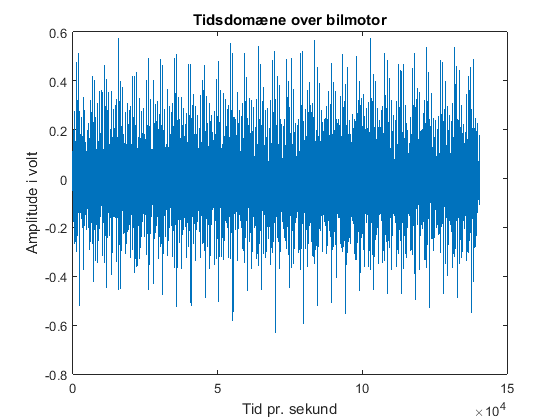
\includegraphics[width=1.1\linewidth]{billeder/bilmotortids}}{\caption{}\label{case1}}
             \ffigbox{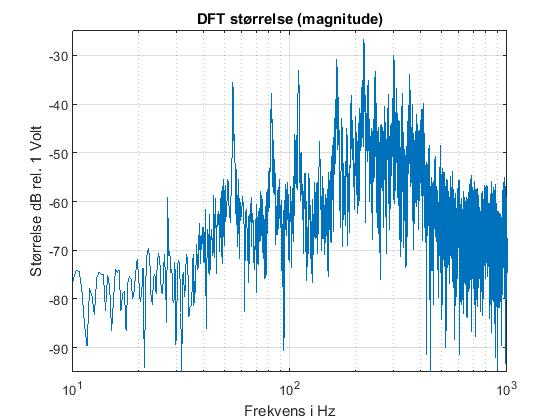
\includegraphics[width=1.1\linewidth]{billeder/storrelsebilmotor}}{\caption{}\label{zoom}}       
           \end{floatrow}
\end{figure}

\begin{center}
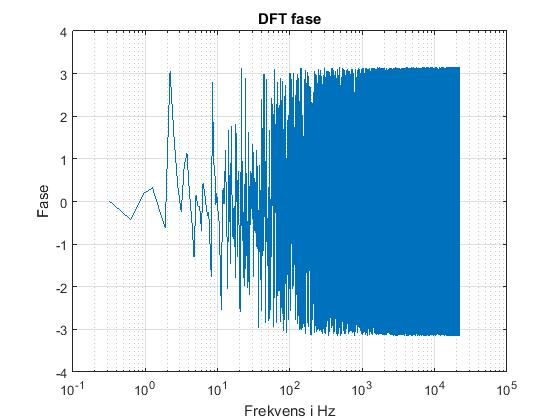
\includegraphics[width=0.55\linewidth]{billeder/fasebilmotor}
\end{center}

Figur 1 er en graf over tidsdomænet. Her ses hvordan amplituden forholder sig i forhold til tiden. Herefter laver vi DFT og transformerer vores signal over i frekvensdomænet. Her laver vi bodeplot - amplitude- og fasekarakteristik over signalet. Figur 2 er vores amplitudespektre - som det kan ses på figur 2 har vi i bilmotorstøjen mest med lavfrekvenser at gøre.  
Figur 3 er fasekarakteristikken, der er ikke det store fasedrej her, så i princippet er figure 3 ikke så interessant. 

\newpage


\subsection{Analyse af vindmøllestøj}
\begin{figure}[!h]
           \begin{floatrow}
             \ffigbox{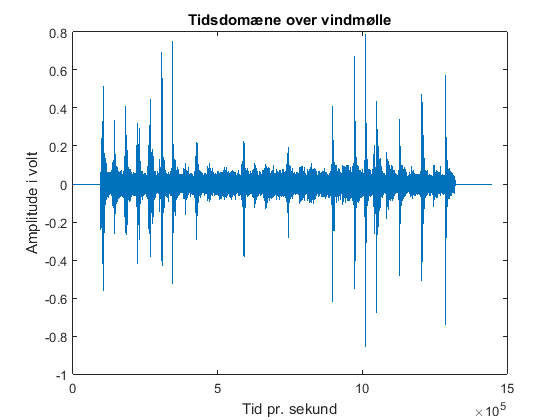
\includegraphics[width=1.1\linewidth]{billeder/vindtid}}{\caption{}}
             \ffigbox{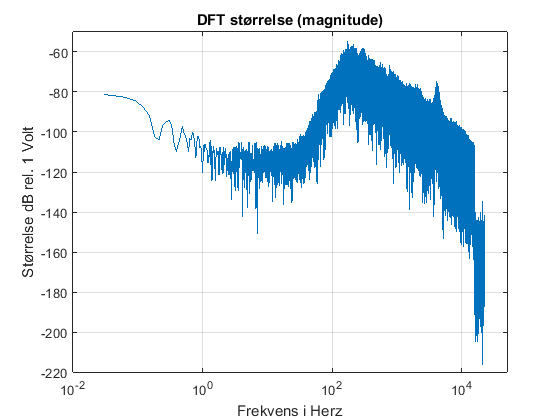
\includegraphics[width=1.1\linewidth]{billeder/vindstorrelse}}{\caption{}}       
           \end{floatrow}
\end{figure}

\begin{figure}[!h]
           \begin{floatrow}
             \ffigbox{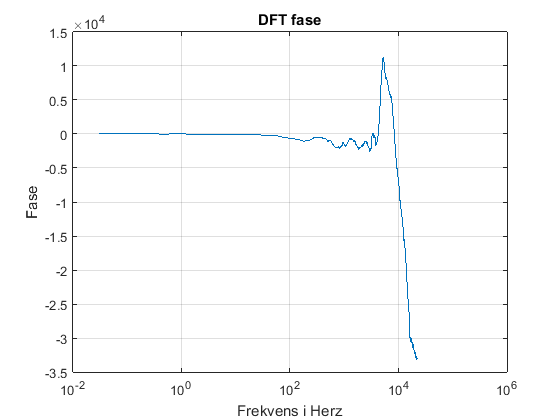
\includegraphics[width=1.1\linewidth]{billeder/vindfase}}{\caption{}}
       
           \end{floatrow}
\end{figure}

Da vindmøllestøj er meget lave frekvenser, er det her smart at køre vores signal igennem et lavpasfilter, så vi netop får filtreret alle de høje frekvenser, der ikke burde være der, fra. Det kunne f.eks. være snak og fuglekvidder. 

\newpage




\subsection{Analyse af EKG}
Da vi her ikke har med et lydsignal at gøre, skal vi ikke længe benytte funktionen "semilogx", men blot funktionen "plot".

\newpage



\subsection{Analyse af Mozart}
Mozart - 39's Symphony no. 40 - 1st movement
\begin{figure}[!h]
           \begin{floatrow}
             \ffigbox{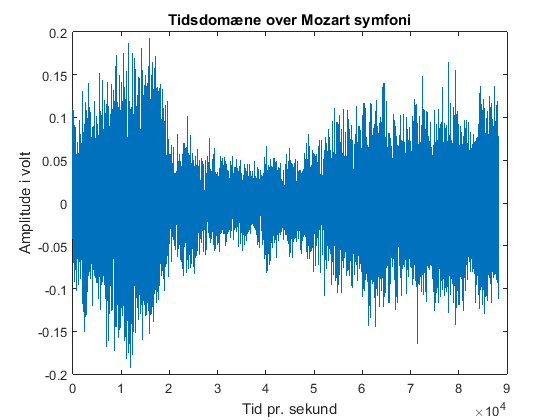
\includegraphics[width=1.1\linewidth]{billeder/mozarttid}}{\caption{}\label{case1}}
             \ffigbox{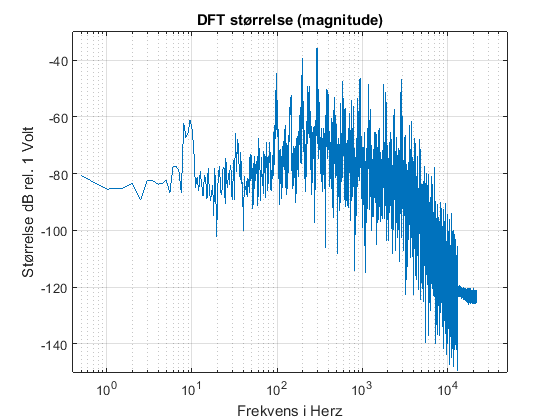
\includegraphics[width=1.1\linewidth]{billeder/mozartstorrelse}}{\caption{}\label{zoom}}       
           \end{floatrow}
\end{figure}


\begin{figure}[!h]
           \begin{floatrow}
             \ffigbox{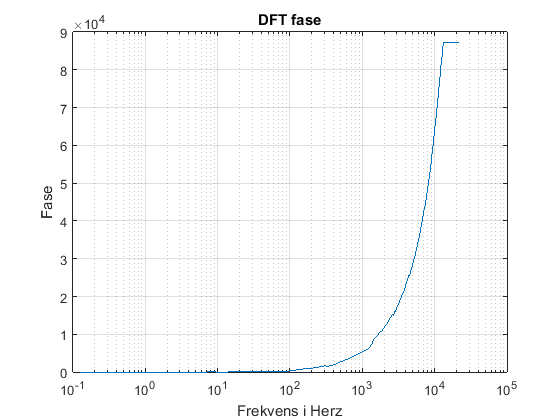
\includegraphics[width=1.1\linewidth]{billeder/mozartfase}}{\caption{}}
       
           \end{floatrow}
\end{figure}

På figur 6 ses Mozarts 39's symfoni i tidsdomænet. Det ses hvordan symfonien udvikler sig over tid. I begyndelsen af udklippet af symfonien er der få instrumenter, der spiller mezzo-piano, så amplituden bliver ikke særlig høj, men efter ca. 1.8 sekunder kommer der flere instrumenter på og de spiller pludselig forte, derfor bliver amplituden højere, hvilket kan ses på figur 6. 
På figur 7 ses amplitudespektret i frekvensdomænet. 
Figur 8 er fasespektret. 

\newpage

\subsection{Analyse af The Weeknd}
The Weeknd - Can't feel my face

\begin{figure}[!h]
           \begin{floatrow}
             \ffigbox{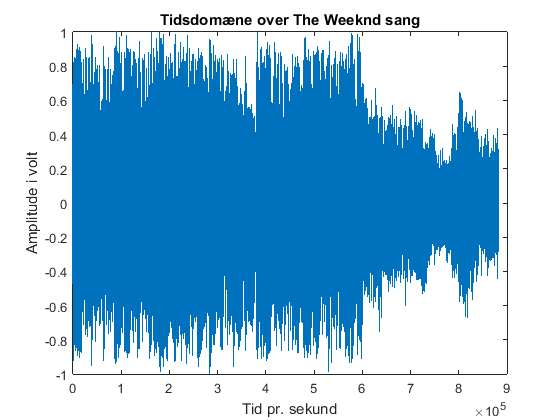
\includegraphics[width=1.1\linewidth]{billeder/weekndtid}}{\caption{}\label{case1}}
             \ffigbox{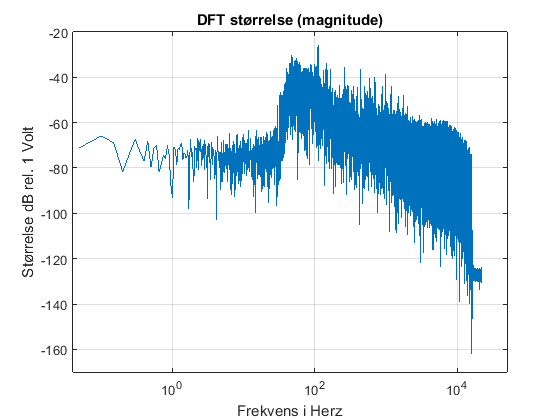
\includegraphics[width=1.1\linewidth]{billeder/weekndstorrelse}}{\caption{}\label{zoom}}       
           \end{floatrow}
\end{figure}

\begin{figure}[!h]
           \begin{floatrow}
             \ffigbox{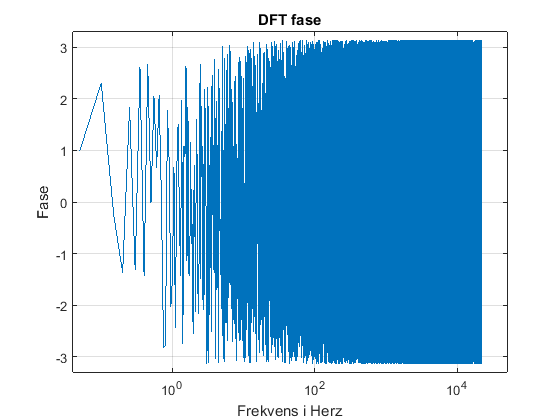
\includegraphics[width=1.1\linewidth]{billeder/weekndfase}}{\caption{}}
       
           \end{floatrow}
\end{figure}

Vi har lige ramt ind i omkvædet af sangen, hvor der er rigtig meget gang i den - efter omkvædet stilner det lidt af igen. Dette kan ses på figur 9, som er vores signal i tidsdomænet. 
Denne sang er rigtig sjov, for The Weeknd kan komme rigtig højt op og det giver os mulighed for at se en hel del høje frekvenser på vores figur 10. 

\newpage


\subsection{Analyse af Eminem}
Eminem - Lose yourself

\begin{figure}[!h]
           \begin{floatrow}
             \ffigbox{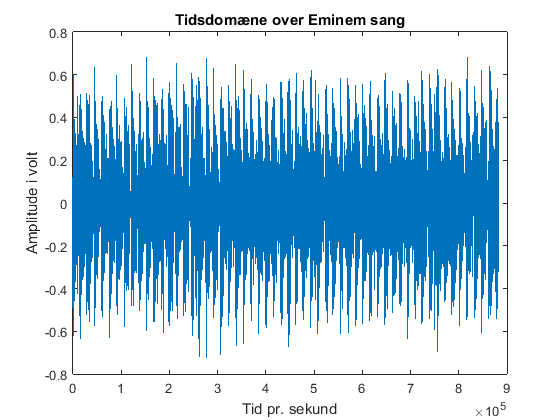
\includegraphics[width=1.1\linewidth]{billeder/eminemtid}}{\caption{}\label{case1}}
             \ffigbox{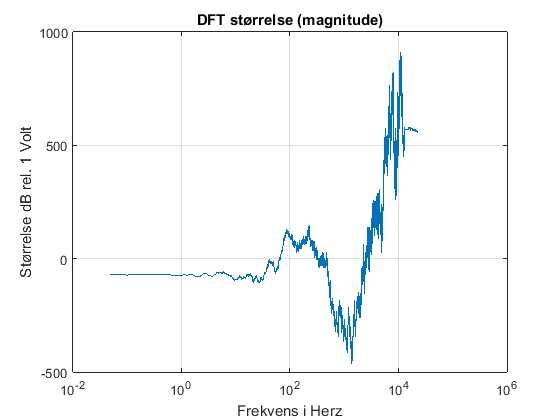
\includegraphics[width=1.1\linewidth]{billeder/eminemstorrelse}}{\caption{}\label{zoom}}       
           \end{floatrow}
\end{figure}

\begin{figure}[!h]
           \begin{floatrow}
             \ffigbox{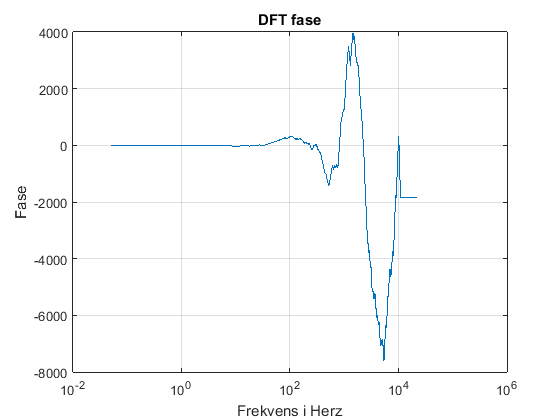
\includegraphics[width=1.1\linewidth]{billeder/eminemfase}}{\caption{}}
       
           \end{floatrow}
\end{figure}


\newpage



\subsection{Analyse af Arctic Monkeys}
Arctic Monkeys - R U Mine

\begin{figure}[!h]
           \begin{floatrow}
             \ffigbox{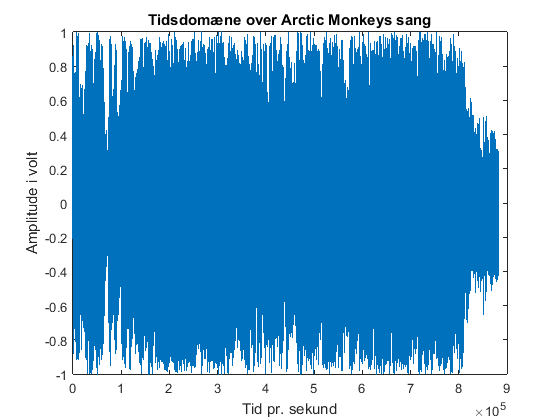
\includegraphics[width=1.1\linewidth]{billeder/arctictid}}{\caption{}\label{case1}}
             \ffigbox{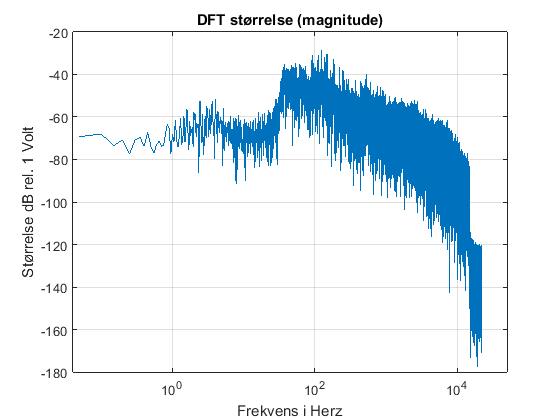
\includegraphics[width=1.1\linewidth]{billeder/arcticstorrelse}}{\caption{}\label{zoom}}       
           \end{floatrow}
\end{figure}


\begin{figure}[!h]
           \begin{floatrow}
             \ffigbox{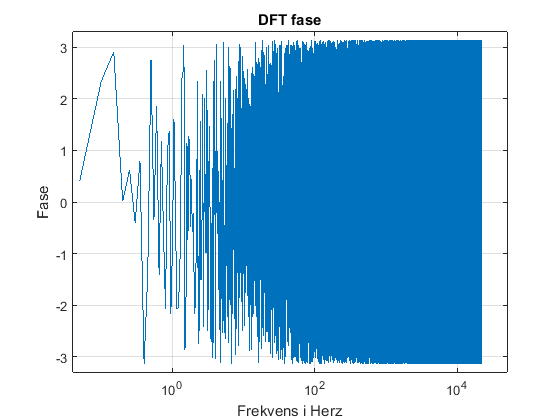
\includegraphics[width=1.1\linewidth]{billeder/arcticfase}}{\caption{}}
       
           \end{floatrow}
\end{figure}


\newpage

\subsection{Analyse af Rednex}
Rednex - Cotton Eye Joe 


\begin{figure}[!h]
           \begin{floatrow}
             \ffigbox{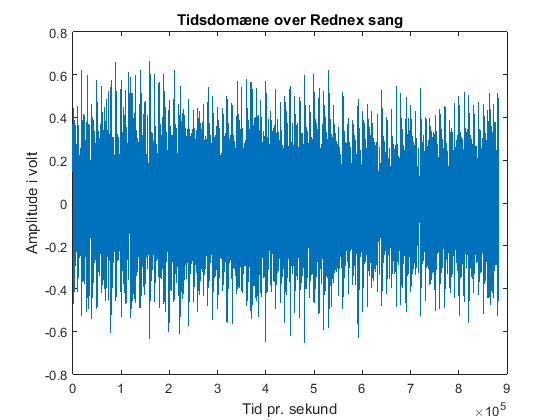
\includegraphics[width=1.1\linewidth]{billeder/rednextid}}{\caption{}\label{case1}}
             \ffigbox{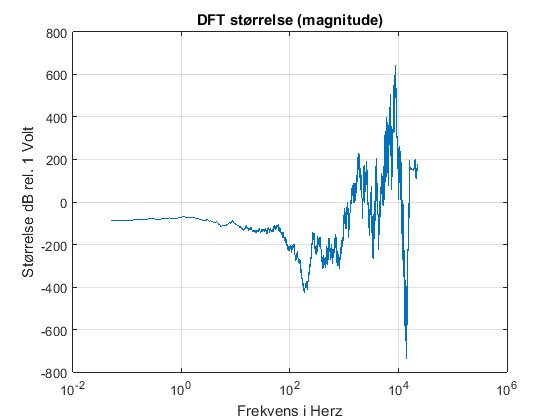
\includegraphics[width=1.1\linewidth]{billeder/rednexstorrelse}}{\caption{}\label{zoom}}       
           \end{floatrow}
\end{figure}

\begin{figure}[!h]
           \begin{floatrow}
             \ffigbox{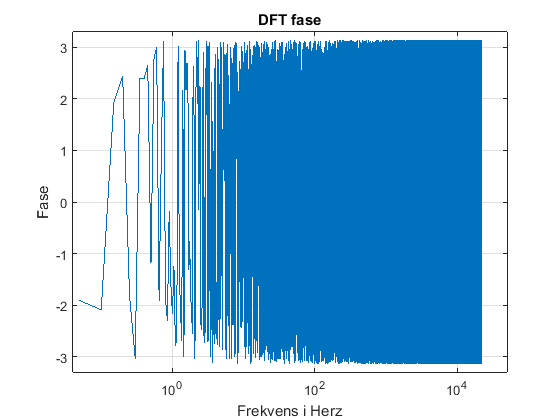
\includegraphics[width=1.1\linewidth]{billeder/rednexfase}}{\caption{}}
       
           \end{floatrow}
\end{figure}



\newpage











\end{document}